\chapter{The 4mm (68-92 GHz) Receiver}\label{chap:wband}
 
%++++++++++++++++++++++++++++++++++++++++++++++++++++++++++++++++++++++++++++

\section{Overview} The 4\,mm receiver (``W-band'') is a dual-beam,
dual-polarization receiver which covers the frequency range of
approximately 67-93 GHz.  The performance degrades significantly
outside of this range.  After the amplifier upgrade in the fall of
2012, typical system temperatures are under 100\,K over much of the
band (Figure~\ref{fig:wperformance}).  A key difference between the
4\,mm receiver and other GBT receivers is that there are no
noise-diodes for the 4\,mm receiver.  This impacts the observing and
calibration techniques for the receiver.  Users need to take a
calibration sequence whenever the configuration changes or whenever
the IF system is balanced for any data that needs to be calibrated.
The receiver has an optical table with an ambient and cold load that
is used for calibration (Figure~\ref{fig:4mmwheel}) .  The optical
table can also convert linear polarization into circular polarization
using a $1/4$-wave plate in front of one of the beams for VLBI
observations.  The two beams are separation by $286^{\prime\prime}$ in
the cross-elevation direction on the sky (i.e., along azimuth).


\begin{figure}[!h]
\begin{center}
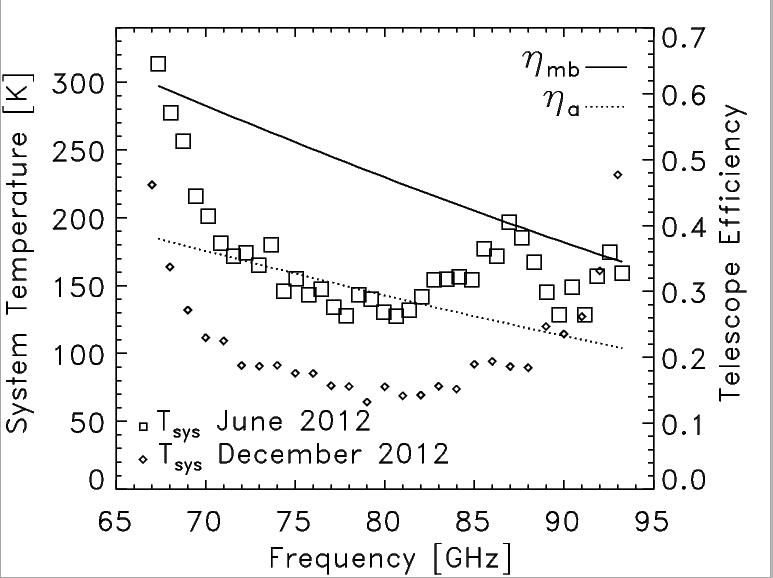
\includegraphics[width=5.0in]{4mm_performance.jpg}
\caption[]{The derived main-beam ($\eta_{mb}$) and aperture
  ($\eta_{a}$) efficiencies from 2012 are given by the solid and
  dotted line respectively.  These estimated efficiencies are based on
  measurements made after an AutoOOF, and the $\eta_{a}$ values are
  slightly less than expected (measurements correspond to surface
  errors of 280$\mu$m instead of the advertised 240$\mu$m errors for
  the dish).  The squares and diamonds show the measured system
  temperatures for the original amplifiers (2012 June) and the upgraded
  amplifiers (2012 December) respectively.  Both sets of data were
  collected under similar conditions with $\tau_o \simeq 0.2$ at 86
  GHz.  \label{fig:wperformance} }
\end{center}
\end{figure}

In this chapter, we present information for carrying out W-band
observations.  We concentrate on items specific to W-band, and assume
the user is familiar with the other chapters of the observing guide.
Contact your support astronomer if you have questions.

\begin{figure}[!h]
\begin{center}
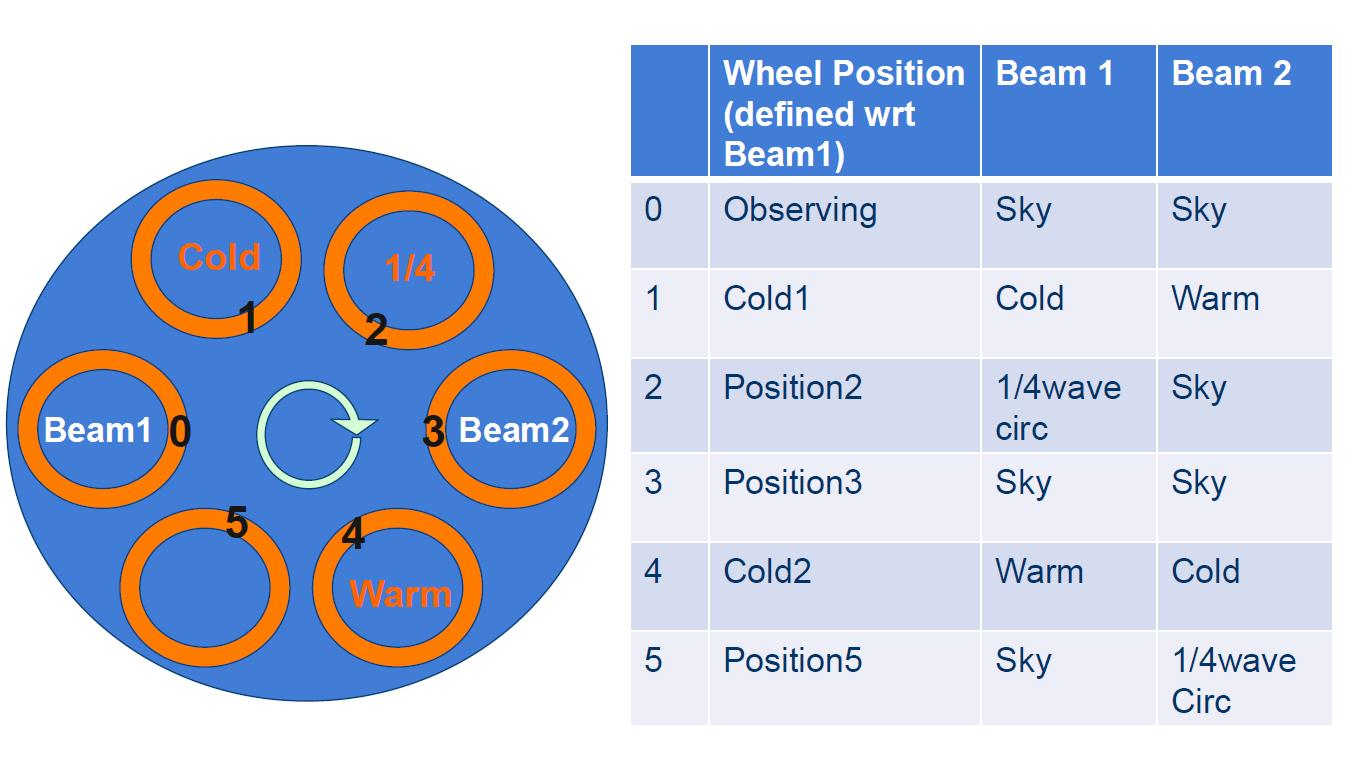
\includegraphics[width=5.0in]{4mm_wheel.jpg}
\caption[]{Diagram showing the positions of the 4mm Calibration wheel.
  The wheel is rotates above the cryostat, and the location of the
  beams are separated by 180 degrees on the wheel.  In the Observing
  position, both beams see the sky.  In the Cold1 position, beam-1
  sees the cold load and beam-2 sees the ambient load, while for the
  Cold2 position, beam-2 sees the cold load and beam-1 sees the
  ambient load. The 1/4-wave plate can be placed over only one of the
  beams at a time.  \label{fig:4mmwheel} }
\end{center}
\end{figure}

\section{Configuration}

The 4mm Receiver uses the standard config-tool software that
automatically configures the GBT IF system based on user input (e.g.,
frequency and bandwidth).  Example w-band configuration files are
given in /home/astro-util/projects/4mm/.  The 4mm system is broken
into into four separate bands:

\begin{itemize}
\item    FL1: 67-74 GHz
\item    FL2: 73-80 GHz
\item    FL3: 79-86 GHz
\item FL4: 85-93 GHz,
\end{itemize}

You can only use one of these bands at a time (i.e., you cannot
simultaneously observe lines in more than one band).  The millimeter
down-converter filters of the system limits the instantaneous
bandwidth to 4 GHz for 73-93 GHz (filters FL2, FL3,FL4), while up to 6
GHz of total bandwidth is available for 67-74 GHz (filter FL1).

The configuration items specific to the 4mm receiver are the following:

\begin{itemize}
\item receiver  = 'Rcvr68\_92'  (name of the receiver)
\item beam      = 'B12', 'B1', or 'B2' (dual beam receiver)
\item swmode    = "tp\_nocal"  or ``sp\_nocal''.  There are no noise
  diodes with this receiver. 
\item polarization = ``linear'' or ``circular'' (Default is linear). If
  user selects circular, then the 1/4-wave plate is placed in front of
  the chosen beam.  There is only one 1/4-wave plate, so users can
  have circular polarization for only one of the beams.
\end{itemize}

\section{Observing}

In general, observations should be carried out during the night under
stable thermal conditions to maximize the observing efficiency for
targets smaller or similar in size to the beam ($\sim
10^{\prime\prime}$).  During the daytime, the effective point-source
aperture efficiency decreases significantly since the beam shape
increases in size.  Depending on the science goals, successful daytime
observations are possible for extended sources.

\begin{itemize}



\item Start the project with an AutoOOF (unless observing extended
  sources during the day).  This sets the active surface, including
  the thermal corrections, as well as getting initial pointing and
  focus corrections.  

\item After configuration and balancing, check the RF power levels in
  the IF rack to confirm that power is going through the channels and
  that the power levels are not saturated ($<10$).  Beam-1 uses
  channels 1 and 3, and beam-2 uses channels 5 and 7.  To avoid
  possible saturation on the warm load, the power levels on the sky
  need to be at $<6$.  Although reasonable looking data may be
  detected downstream, observers should avoid non-linear calibration effects
  when the IF power saturates (RF Power $=10$), and special care should
  be taken in calibration of such data.  The target power level for
  w-band is 1.5, and the software adjusts the attenuation to reach
  this level.  If the channel(s) are saturated with maximum
  attenuation (31dB), users can decrease the bandwidth of the
  observations (e.g., avoid using ``All Pass'' or choose a smaller
  filter to decrease the power levels).  If the channels(s) do not
  have enough power with the no attenuation (0dB), users can increase
  the filter bandwidth or choose ``All Pass'' to increase the power
  levels.  In general, manual changes of the default configuration
  values for the IF rack should not be needed for most configurations.

\item Users must run the CalSeq procedure to calibrate the data (see
  \S~\ref{sec:calseq}).  During the calibration sequence, users can
  watch the movement of the calibration wheel from the Rcvr68\_92 cleo
  page (Figure~\ref{fig:4mmrxcleo}).

\end{itemize}

\subsection{CalSeq}\label{sec:calseq}

The CalSeq procedure is used to calibrate w-band data.  This procedure
should be run after every configuration and balance.  This is needed
to convert instrumental voltages into antenna temperatures.  The
syntax for the Calseq command is the following:

{\bf CalSeq}(type, scanDuration, [location, beamName, fixedOffset,
tablePositionList, dwellFractionList]), where the arguments in [ ]
are optional.

\begin{itemize}

\item  type: string keyword to indicate type of calibration scan: manual,
  auto, autocirc

\begin{itemize}
        
\item "manual" -- A separate scan will be done for each table
  position. The user can input a list of calibration table wheel
  positions with the tablePositionList argument.

\item "auto" -- default dwell fraction =(0.33, 0.33, 0.34) and default
  three positions = (Observing, Cold1, Cold2). The user can specify a
  list of positions and dwell times with the tablePostionList and
  dwellFractionList arguments.
        
\item "autocirc" -- dwell fraction =(0.25, 0.25, 0.25, 0.25) and four
  positions = (Observing, [Position2 for beamName='1' or Position5 for
  beamName='2' for use with circular VLBI observations], Cold1,
  Cold2).

\end{itemize}


\item scanDuration: scan exposure time, in seconds. For manual mode,
  each specified position will be observed for the scan exposure time
  (i.e., separate scans for each position). For auto modes, the total
  scan exposure time will be divided between positions based on the
  dwell fractions (i.e., one scan for all positions).

\item location: a Catalog source name or Location object; default is
  None (use current location).
    
\item beamName: Beam name associated with pointing location. This
  argument is a string. Default beam is '1'.
    
\item fixedOffset: offset sky position (used in cases when observing a
  bright source and want to measure the system temperature of the sky
  off-source). This argument should be an Offset object. Default sky
  offset is 0.
    
\item tablePositionList: user-specified, variable-length ordered list
  of cal table positions for the manual or auto modes.  The default
  sequence is ['Observing', 'Cold1', 'Cold2'].
    
\item dwellFractionList: user-specified, ordered list of dwell
  fractions associated with the tablePositionList for use only with
  the auto mode. By using auto mode with tablePositionList and
  dwellFractionList, expert users can control the wheel in any order
  of positions and dwell fractions. This input not needed for autocirc
  or manual modes is ignored in these modes if given.

\end{itemize}

Example usage of the CalSeq command:

\begin{itemize}

\item CalSeq(``auto'',40.0).  This command can be used for most
  observations, which uses the default tablePositionList=['Observing',
  'Cold1', 'Cold2'].

\item CalSeq(``auto'',40.0,fixedOffset=Offset(``J2000'', ''00:00:00'',
  ''00:02:00'')).  This command can be used for bright objects where
  one wants a system temperature measurement on blank sky.  In this
  example, the offset is $2^{\prime}$ to the north.  If observing a
  large object, one can increase the offset size to move off-source
  for the blank-sky measurement.

\item CalSeq(``manual'',10.0,tablePositionList=['Position2',
  'Observing', 'Cold1', 'Cold2']).  This is an example command for
  calibration of VLBI observations with beam-1 circular polarization.
  We can only observe the cold and ambient loads with linear
  polarization.  The calibration from linear to circular requires
  observations of the same sky with both linear and circular
  polarization (Observing and Position2, respectively, in this
  example).

\end{itemize}


\begin{figure}[!h]
\begin{center}
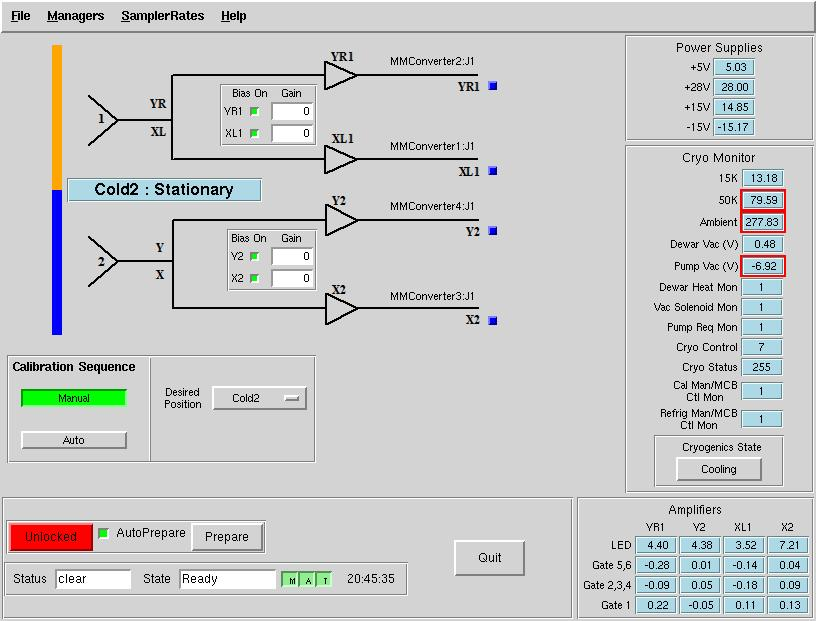
\includegraphics[width=5.0in]{4mm_Rx_cleo.jpg}
\caption[]{The 4mm Receiver CLEO window.  Users can manual move the
  wheel by using the ``Desired Position'' button.  The temperature of
  the ambient load used for calibration is given by the ``Ambient''
  temperature sensor value shown at the right (277.83 K in this
  example). \label{fig:4mmrxcleo} }
\end{center}
\end{figure}

\subsection{Pointing and Focus}

Blind pointing at the start of the observing run may not be successful
since the blind pointing errors can be similar to the beam size, and the
source may be missed in the simple Az-El scans used by the Peak
procedure.  Initial pointing offsets can be found with the AutoOOF
procedure, or users may want to point on Jupiter or another large
source as needed.  Pointing and focus for W-band requires special
attention, and users should not blindly accept the default solutions
provided by the software system.  Users can enter solutions manually
as needed as discussed in Section~\ref{sec:gfmsendcorrections}.

 
\subsection{AutoOOF Thermal Corrections}

Optimal point-source observations should be carried out with regular
AutoOOF measurements (every 2-4 hours) during the nighttime when the
thermal stability of the dish is best.  Based on commissioning tests
with the 4mm receiver, the AutoOOF corrections improves the
point-source aperture efficiency by 30--50\%.  Application of these
corrections during the day are typically not practical for the 4mm
receiver given the thermal environment of the dish is generally not
sufficiently stable.  During the day, the measured beam sizes can vary
significantly (e.g., 10--$14^{\prime\prime}$), but the beam shape
typically remains well-behaved (fairly symmetric and Gaussian).
Although the variation of beam size has a direct impact on the
point-source aperture efficiency ($\eta_{a}$), it has less of an
impact on the effective main-beam efficiency ($\eta_{mb}$) used for
the calibration of extended sources.  For example during the
commissioning of the instrument, we measured a beam size of
$10.8^{\prime\prime}$ at 77 GHz and derived $\eta_{a} = 31$\% and
$\eta_{mb}=50$\% in good nighttime conditions with the application of
the thermal AutoOOF corrections.  Without the AutoOOF corrections, the
beam-size increased to $12.5^{\prime\prime}$ and the aperture
efficiency decreased to 23\%, but the main-beam efficiency remained
nearly constant at about 50\% ($\eta_{mb} \propto \theta_{mb}^2
\eta{a}$).  Therefore, extended sources may be observed during the day
without the AutoOOF corrections if the science is not impacted by the
primary beam variations.

\section{Calibration and Data Reduction}


For accurate calibration, users are recommended to run a CalSeq before
and after each set of source data.  Users are also recommended to take
a short nod observation on their pointing \& focus source every hour
to track the relative efficiency of the system.  If users only want
absolute calibration done to within 20--30\%, then the default
calibration from the cold\&ambient loads may be used.  For more
accurate absolute flux calibration, a source of known flux density
should be used.  The ALMA Calibrator Source Catalogue has an extensive
record of the flux density histories for many of the bright 3mm point
sources (https://almascience.eso.org/sc/).  By using ALMA flux density
values as a function of time, $\sim$10\% absolute calibration
uncertainties can be obtained for W-band data.

\begin{table*}
%  \vspace{0.0cm}
\begin{center}
    \caption{4mm Channel Definitions}
    \begin{tabular}{lrr}
      \hline 
      \hline 
      \multicolumn{1}{l}{Channel} &
      \multicolumn{1}{c}{Polarization} & 
      \multicolumn{1}{c}{Beam}\\
      \hline

ch1& beam1 (fdnum=0) & X or L (plnum=0)\\
ch3& beam1 (fdnum=0) & Y or R (plnum=1)\\
ch5/6& beam2 (fdnum=1) & X or L (plnum=0)\\
ch7& beam2 (fdnum=1) & Y or R (plnum=1)\\
  \hline 
   \end{tabular}
\end{center}

\noindent{\bf Table Notes:} The GBT IF channel numbers 1,3,5,7 and
their corresponding beam and polarization definitions.  The parameters
fdnum and plnum are GBTIDL keywords.
\end{table*}

The standard GBTIDL scripts (getps, getnod, getfs) do not work since
these assume a noise diode for calibration. W-band scripts for the
reduction of spectral line data can be found at
/home/astro-util/projects/4mm/PRO. For continuum (DCR) reduction,
contact your support scientist.  Users can use the calseq.pro within
GBTIDL to derive the gains for each of the channels.  After deriving
the gains, users can and reduce the spectra-line data, for example,
using wonoff\_gain.pro.

The formulae for calibrating data are given below.  The observed
antenna temperature is

\begin{equation}
T_{A} = T_{\rm sys} (V_{ON} - V_{OFF})/V_{OFF},
\end{equation}
where  $V_{ON}$ and
$V_{OFF}$ are the observed voltages of the ON and OFF scans. 
The system temperature ($T_{\rm sys}$) is given by 
\begin{equation}
  T_{\rm sys} = g\,V_{OFF}, 
\end{equation}
and the gain ($g$) is
\begin{equation}
g = [(T_{amb}-T_{cold})/(V_{amb} - V_{cold})],
\end{equation}
where $T_{amb}$ and $T_{cold}$ are the temperatures of the ambient and
cold loads and $V_{amb}$ and $V_{cold}$ are the observed voltages of
the ambient and cold load scans.  The ambient load is given on the
receiver CLEO page and within the receiver FITS files.  The cold load
is measured in the lab (Table~18.2).  The main-beam temperature
$T_{mb}$ is related to the observed antenna temperature $T_{a}$ by
\begin{equation}
T_{mb} = T_{A} \exp(\tau_{o}A)/\eta_{mb},
\end{equation}
where $\tau_{o}$ is the zenith opacity and $A$ is the airmass.
Assuming a Gaussian beam, the main-beam efficiency is given by
\begin{equation}
\eta_{mb} = 0.8899\eta_{a}(\theta_{FWHM} D/\lambda)^2,
\end{equation}
where $\theta_{FWHM}$ is the full-width half-maximum beam size in
radians, D is the diameter of the GBT (100m), and $\lambda$ is the
observed wavelength. For the GBT, the effective aperture efficiency is
\begin{equation}
\eta_{a} = 0.3516 T_{A} \exp(\tau_{o}A)/S_{\nu}, 
\end{equation}
where $S_{\nu}$ is the flux density of a known calibration source.

The opacity as a function of time can be obtained by the weather
database derived for Green Bank using the getatmos.pro script.  Except
for periods of rapidly changing weather conditions, the predicted
opacities are accurate to within $\Delta \tau_o \simeq 0.01$ based on
historical measurements.



\section{Web Documentation}

\begin{itemize}

\item 4mm Web Page: http://www.gb.nrao.edu/4mm/

\item 4mm Project Book: http://www.gb.nrao.edu/4mm/ProjectBook/

\item 4mm Wiki: https://safe.nrao.edu/wiki/bin/view/GB/Gbt4mmRx

\item 4mm Status and Commissioning Wiki which provides latest info on
  performance and notes for users:
https://safe.nrao.edu/wiki/bin/view/GB/Gbt4mmRxCommissioning

\end{itemize}


\begin{table*}
%  \vspace{0.0cm}
\begin{center}
    \caption{Effective Cold Load Temperature for W-band}
    \begin{tabular}{lc}
      \hline 
      \hline 
      \multicolumn{1}{l}{Date Range} &
      \multicolumn{1}{c}{Average Temperature}\\
      \hline
2010 May -- 2012 April & 53 K\\
2012 May -- 2012 June  & 56 K\\
2012 October -- 2015 August  & 50 K\\
2015 September -- & 54 K\\
  \hline 
   \end{tabular}
\end{center}
   
\noindent{\bf Table Notes:} The estimated effective cold load
temperature measured in the lab.  The temperature is estimated to
better than $\pm$5\,K.  Note, that a 10\% error in the cold load
measurement corresponds to only about a 2.5\% error in the measured
$T_{a}$ or $\eta_{a}$.

\end{table*}
